% !TEX root = ../thesis_main.tex
\chapter{Properties of Single-Wall Carbon Nanotubes}

The properties of carbon nanotubes (CNTs) strongly depend on their crystal structure. CNTs consist of carbon atoms bound together via sp$^2$ orbitals ($\sigma$ bonds) and arranged in a honeycomb lattice \cite{soavi2016ultrafast}. They can exist as single-wall carbon nanotubes (SWCNTs), double-wall carbon nanotubes (DWCNTs), and multi-wall carbon nanotubes (MWCNTs) as depicted in Figure \ref{fig:swcnt_mwcnt}. DWCNTs are comprised of two concentric nanotubes. Whereas, MWCNTs contain more than two concentric nanotubes. Nevertheless, this thesis focuses on the properties of SWCNTs. 

\begin{figure}[ht]
	\centering
	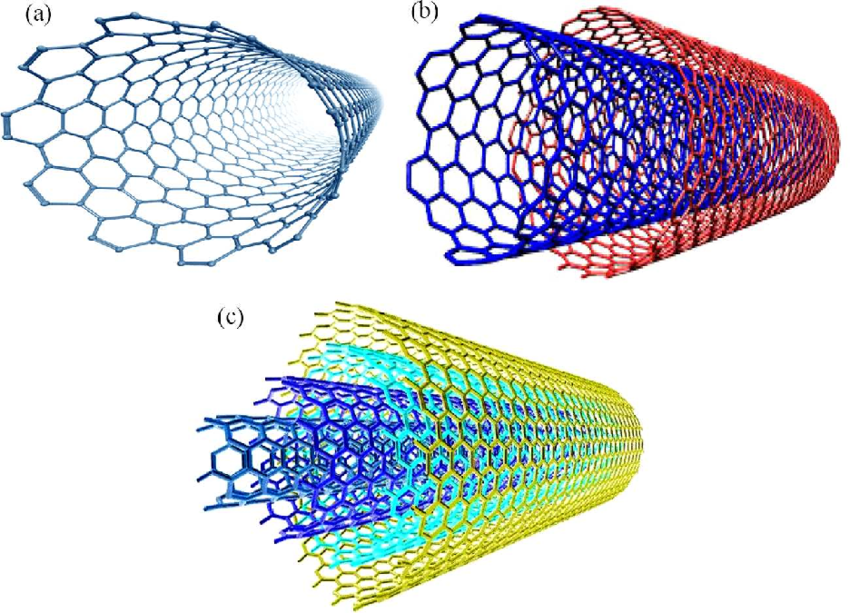
\includegraphics[scale=1]{images/chapter_optical_props/swcnt_mwcnt_rafiq}
	\caption{Schematic diagram showing the crystal structures of (a) a single-wall carbon nanotube , (b) a double-wall carbon nanotube  and (c) a multi-wall carbon nanotube. Reproduced from Ref.\ \cite{rafique2016exploration}.}
	\label{fig:swcnt_mwcnt}
\end{figure}

Due to the similarities between the crystal structures of graphene and SWCNTs, different SWCNT species can be classified using the basis vectors of the graphene lattice \cite{charlier2007electronic}. In fact, the countless ways of rolling up a graphene sheet into a nanotube evince that CNTs can exhibit varying helical geometries and symmetries with respect to their axial direction, as shown in Figure \ref{fig:symmetries}.

\begin{figure}[h]
	\centering
	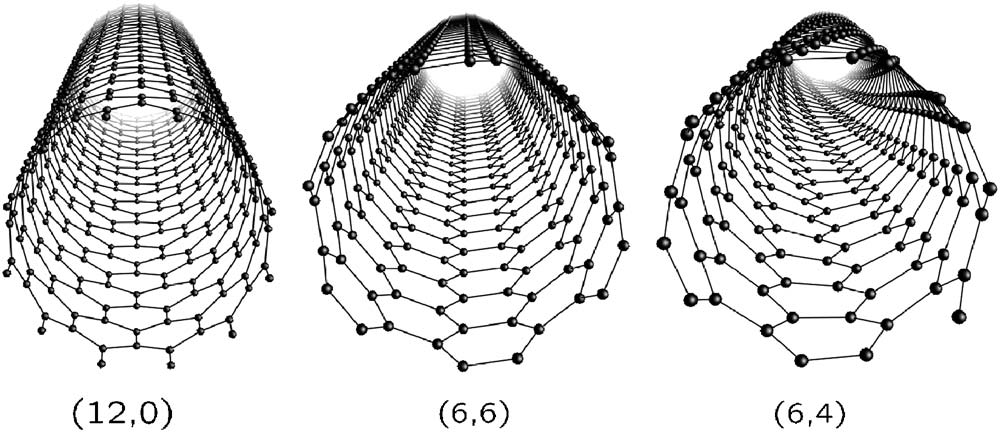
\includegraphics[scale=0.4]{images/chapter_optical_props/nanotube_symmetries_charlier}
	\caption{Crystal structures of (12,0), (6,6) and (6,4) single-wall carbon nanotubes. Reproduced from Ref. \cite{charlier2007electronic}.}
	\label{fig:symmetries}
\end{figure}
These morphological properties dictate the allowed electronic states by asserting boundary conditions on the electron wavefunction along the circumferential direction \cite{charlier2007electronic}. All allowed electronic states exhibit anisotropic features and obey a set of optical selection rules that govern allowed inter-band transitions. Moreover, the effect of strong electron-electron interactions effectively suppress the oscillator strengths associated with optical transitions involving any free-electron continuum states \cite{ando1997excitons}. This behavior distinguishes carbon nanotubes from conventional bulk semiconductors as they typically exhibit relatively weak Coulomb interactions \cite{ando1997excitons}.


\section{Definition of the Chiral Vector $\vec{C}_\text{h}$}

Each unique species of carbon nanotubes can be denoted using a set of indices ($m$,$n$). These integers $m$ and $n$ define the chiral vector $\vec{C_\text{h} }$ expressed as
\begin{equation}
	\vec{C_\text{h}} = n {\vec{a_\text{1}}} + m {\vec{a_2}} \equiv (m,n)
	\label{eq:chiral_vec}
\end{equation}
where $\vec{a_\text{1}}$ and $\vec{a_\text{2}}$ represent the lattice basis vectors of the 2D graphene sheet as shown in Figure \ref{fig:chiral_vectors}. This chiral vector $\vec{C_h}$ yields the nanotube diameter $d_t$ via the expression
\begin{equation}
	d_\text{t} = \dfrac{|\vec{C_\text{h}}|}{\pi} = \dfrac{a_\text{C-C}}{\pi}\sqrt{3(m^2 + mn + n^2)},
\end{equation}
where $a_\text{C-C} \approx$ \SI{1.44}{\angstrom} defines the nearest-neighbor distance between carbon atoms in graphene \cite{nanot2013single}.

\begin{figure}[ht]
	\centering
	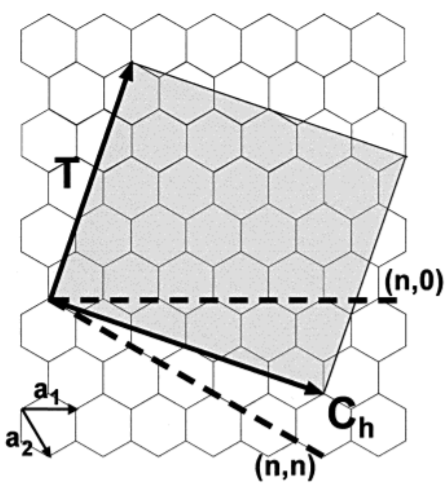
\includegraphics[scale=1]{images/chapter_optical_props/chiral_vectors_sheet.png}
	\caption{Two-dimensional graphene sheet featuring the lattice vectors $\vec{a_1}$ and $\vec{a_2}$ and the chiral vector $\vec{C_h}$ defined in Eq. \ref{eq:chiral_vec}. The vector $\vec{T}$ points in the axial direction of the carbon nanotube. Furthermore, $(n,n)$ and $(n,0)$ represent limiting cases for $\vec{C_h }$. Reproduced from Ref. \cite{odom2000structure}.}
	\label{fig:chiral_vectors}
\end{figure}


\section{Optical and Electronic Properties}

\subsection{Electronic Band Structure}

Given the similarities between CNTs and graphene, calculating the electronic band structure of graphene is the first step towards determining that of CNTs. A simple tight-binding model can be used to calculate the band structure of graphene. Such a model includes first nearest-neighbor interactions involving the $\pi$-orbitals of two atomic sites located at positions and $\vec{a}_1$ as well as $\vec{a}_2$ \cite{charlier2007electronic}. Here, $\vec{a}_1$ and $\vec{a}_2$ represent the lattice vectors of graphene. Furthermore, a hopping term $\gamma_0 \approx 2.9$ eV  characterizes the interactions between neighboring $\pi$-orbitals \cite{charlier2007electronic}. The Hamiltonian $\mathcal{H}$ for this simple system is then written as
%
\begin{equation}
	\mathcal{H} = \begin{bmatrix}
	0 & \alpha(k) \\
	\alpha^*(k) & 0
	\end{bmatrix}
\end{equation}
%
where $\alpha(\vec{k}) = (1 + e^{-i \vec{k}\cdot \vec{a_1}} + e^{-i \vec{k}\cdot \vec{a_2}})$ and $\alpha^*(\vec{k})$ refers to the complex conjugate of $\alpha(\vec{k})$\cite{charlier2007electronic}. In addition, $\vec{k}$ stands for a reciprocal space vector within the first Brillouin zone. Diagonalizing this matrix yields the energy dispersion
%
\begin{equation}
	E^{\pm} (k_\text{x}, k_\text{y}) = \pm \gamma_0 \sqrt{1 + 4 \cos\dfrac{\sqrt{3}k_\text{x} a}{2}\cos\dfrac{k_\text{y} a}{2} + 4 \cos^2 \dfrac{k_\text{y} a}{2}}
	\label{eq:graphene_band}
\end{equation}
 where $E^-$ and $E^+$ stand for the dispersion relations of the valence and conduction bands respectively. The variables $k_\text{x}$ and $k_\text{y}$ denote the x- and y-components of $\vec{k}$. Moreover, the constant $a = \sqrt{3}a_\text{C-C}$, where $a_\text{C-C} \approx$ \SI{1.44}{\angstrom} and refers to the nearest-neighbor distance between the lattice sites.
%
\begin{figure}[h]
	\centering
	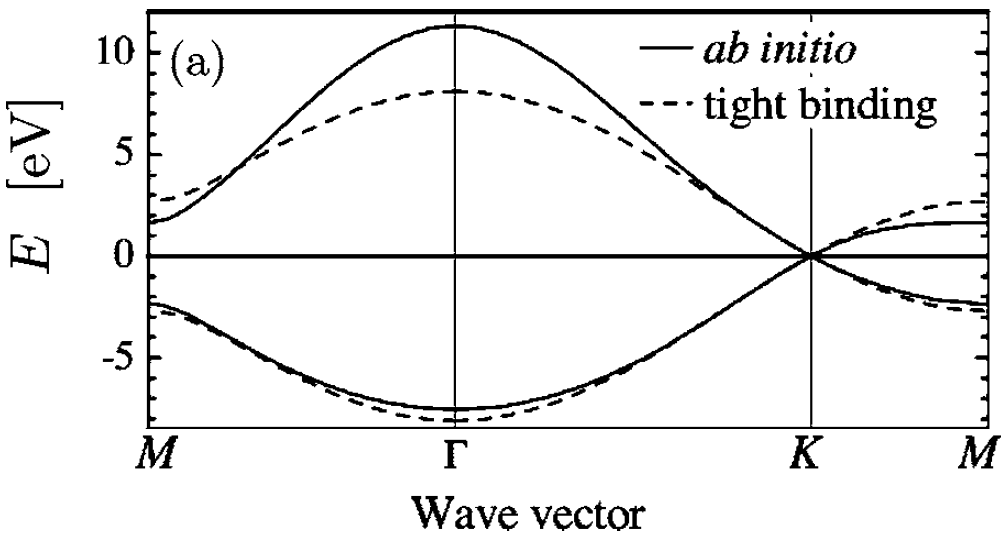
\includegraphics[scale=0.5]{images/chapter_optical_props/graphene_band_charlier}
	\caption{Electronic band structure of graphene determined using a tight-binding model (dashed line) and through ab-initio calculations (solid line). Reproduced and modified from Ref. \cite{reich2002tight}.}
	\label{fig:graphene_band}
\end{figure}
%
Figure \ref{fig:graphene_band} presents a plot of Eq. \ref{eq:graphene_band} as compared with a band structure calculation using ab-initio methods. Despite the disagreement between both approaches, they both predict a linear dispersion in the region near the $K$ position in momentum space \cite{charlier2007electronic}. This region of the band structure is commonly referred to as the Dirac cone	as shown in Figure \ref{fig:dirac_cone} \cite{charlier2007electronic}. In this region , the energy dispersion approximately becomes
\begin{equation}
	\displaystyle E^{\pm}(\vec{q}) \approx \pm v_\text{F}|\vec{q}|
\end{equation}
where $\vec{q}$ is the momentum vector measured with respect to the K point. Furthermore the variable $v_\text{F}$ is the Fermi velocity defined as $v_\text{F} = 3 \gamma_0 a_\text{C-C}/2 \approx 10^6$ m/s. Moreover, both models identify graphene as a semi-metal since the valence and conduction bands intersect at the $K$ point \cite{charlier2007electronic}. Without the presence of any dopants, the Fermi level remains exactly at the position where the two bands cross at the $K$ point and the Fermi surface becomes an infinitesimal point. In conjunction with the band structure of graphene, the zone-folding approximation yields the band structure of CNTs.

\begin{figure}[ht]
	\centering
	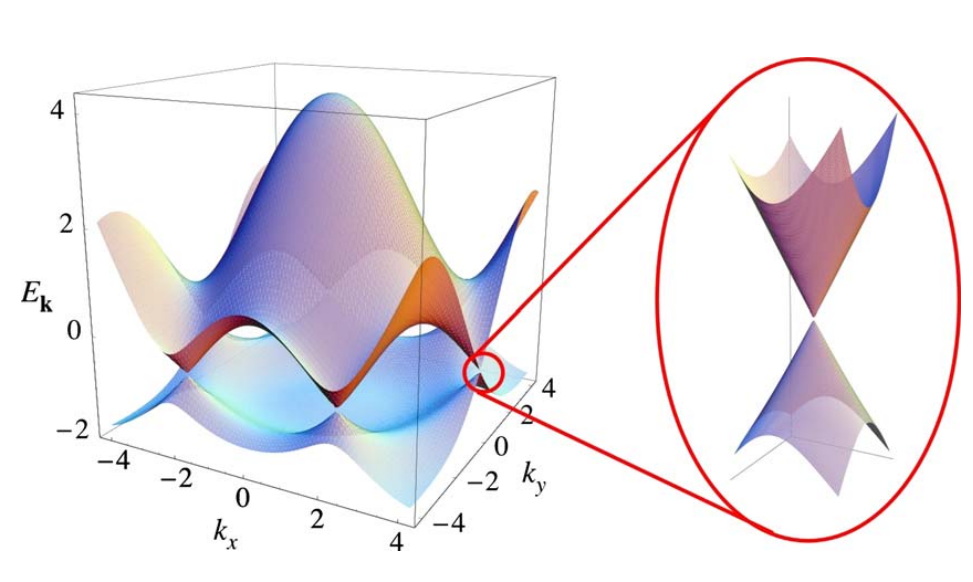
\includegraphics[scale=0.4]{images/chapter_optical_props/dirac_cone}
	\caption{Electronic band structure of graphene with energy in units of $\gamma_0$. Close to the $K$ point, the dispersion becomes approximately linear in a region known as the Dirac cone. Reproduced from Ref.\ \cite{neto2009electronic}.}
	\label{fig:dirac_cone}
\end{figure}


\subsection{Chiralities of Semiconducting and Metallic Nanotubes}

\begin{figure}[ht]
	\centering
	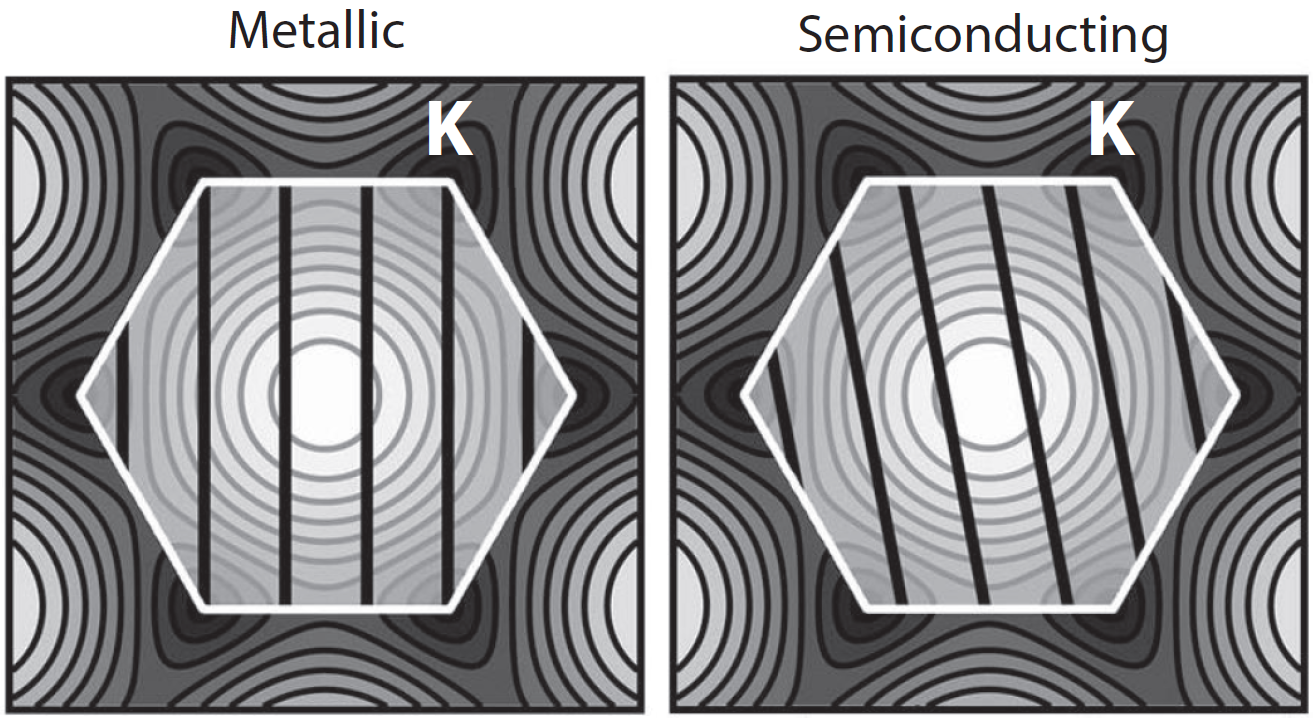
\includegraphics[scale=0.35]{images/chapter_optical_props/metal_semi_amori}
	\caption{The image shows the first Brillouin zone of graphene (white hexagon) superimposed on a countour map of the electronic band structure of graphene. The Dirac cone sites at the K point. Allowed values of $\vec{k}$ according to the quantization condition defined in Eq.\ \ref{eq:quantization_cond} are drawn over the Brillouin zone as thick, black, vertical lines. For metallic nanotubes, the electronic states located at the Dirac cone are allowed. Whereas, the band structures of semiconducting nanotubes do not include a Dirc cone. Reproduced from Ref.\ \cite{amori2018excitons}.}
	\label{fig:k_quant}
\end{figure}

The zone-folding method asserts that the periodic boundary conditions along the circumferential direction of CNTs dictate the quantization of the allowed $\vec{k}$ vectors in the electronic band structure \cite{charlier2007electronic}. This condition applied to the electron wavefunction $\Psi(\vec{r})$ is expressed as
\begin{equation}
\Psi_{\vec{k}}(\vec{r} + \vec{C_\text{h}}) = e^{i \vec{k} \cdot \vec{C_\text{h}}} \Psi_{\vec{k}}(\vec{r}) = \Psi_{\vec{k}}(\vec{r}),
\label{eq:boundary_cond}
\end{equation}
where $\vec{r}$ and $\vec{k}$ respectively define vectors in real and reciprocal space on the surface of the CNT \cite{charlier2007electronic}. Furthermore, $\vec{C_\text{h}}$ represents the chiral vector defined in Eq. \ref{eq:chiral_vec}. This condition gives the quantization of $\vec{k}$ which can be written as
\begin{equation}
	\vec{k} \cdot \vec{C}_h = 2\pi n
	\label{eq:quantization_cond}
\end{equation}
where n is an integer. Equation \ref{eq:quantization_cond} reveals that the symmetry of the CNT given by the chirality $\vec{C_\text{h}} \equiv (n,m)$ determines the band structure. Figure \ref{fig:k_quant} illustrates this. Depending on the chirality of the nanotube, the Dirac cone located at the K point may or may not be included the nanotube's bandstructure. This may determine whether or not the nanotube has a finite band gap energy.



In addition, the variable $\nu$ defined as
%
\begin{equation}
\label{eq:nu_cnt}
\nu \equiv (n-m) \mathrm{\hspace{1.5mm} mod \hspace{1.5mm}} 3,
\end{equation}
%
is also used to classify the two different band structures can occur.
%
\begin{figure}[h]
	\centering
	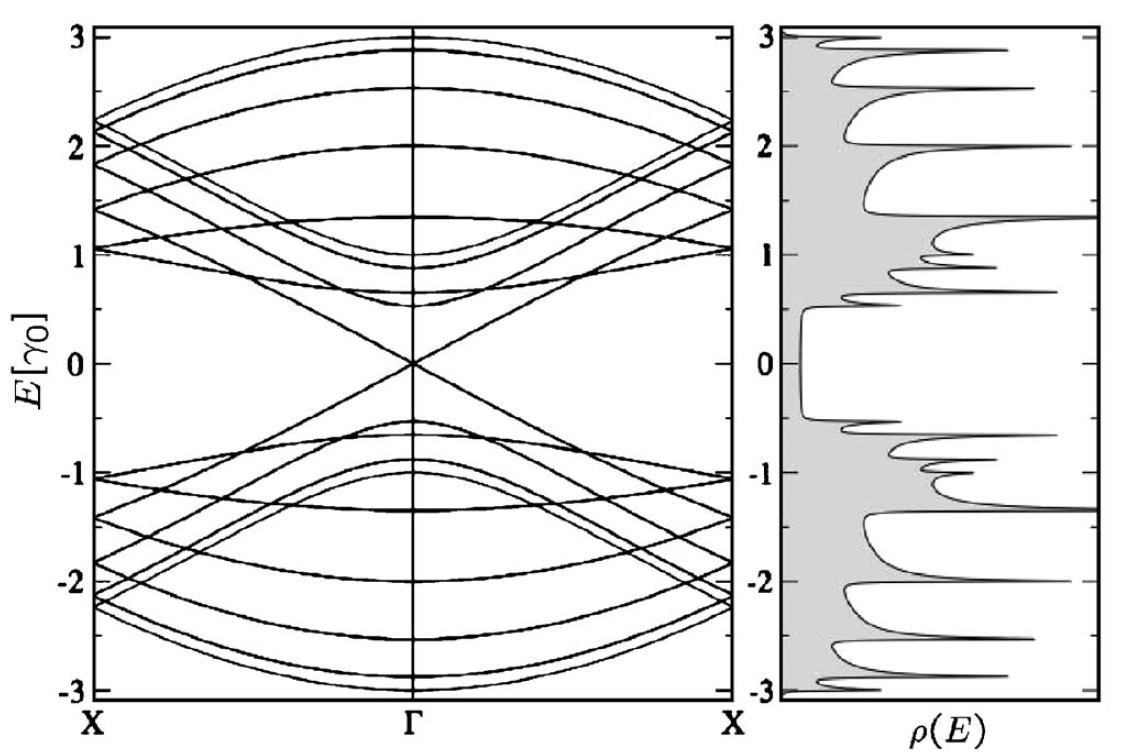
\includegraphics[scale=0.36]{images/chapter_optical_props/nine_zero_band_charlier}
	\caption{Band structure and density of states for a (9,0) carbon nanotube derived using the zone-folding scheme. These are plotted in units of $\gamma_0 \approx 2.9$, the tight-binding hopping energy between first nearest-neighbors. Reproduced from Ref.\ \cite{charlier2007electronic}.}
	\label{fig:nine_zero_cnt}
\end{figure}
%
In the case where $\nu = 0 $, the band structure contains a Dirac cone along with additional sub-bands within the valence and conduction bands as presented in Figure \ref{fig:nine_zero_cnt} . CNTs that satisfy this condition include $(n,n)$ carbon nanotubes, also commonly referred to as ``armchair'' nanotubes, that constitute the set of all metallic (gapless) nanotubes \cite{nanot2012optoelectronic}. Furthermore, $(n,m)$ nanotubes where $n-m = 3j$ ($j > 0$) also satisfy this $\nu = 0$ condition. However, these non-armchair nanotubes ($n\neq m$) exhibit curvature-induced band gaps and can behave as narrow-gap semiconductors ($\sim1 - 100$ meV band gap energy) \cite{nanot2012optoelectronic}.

Curvature most directly refers to the diameter of the carbon nanotube \cite{blase1994hybridization}. It can influence the tendency of anti-bonding $\sigma^*$ and $\pi^*$ orbitals to hybridize, which can add further modifications to the band structure \cite{blase1994hybridization}. These effects are not fully accounted for in the zone-folding scheme.

Figure \ref{fig:cnt_curvature} demonstrates this effect on the band structure of a (6,0) nanotube. The tight-binding model presented in the plots includes the effects of $\sigma^*$ and $\pi^*$ hybridization that manifest the presence of two new states whose difference in energy is determined by the nanotube diameter. At lower diameters, the lower energy band gradually gets closer to the valence band. In a full ab-initio calculation, this band would instead intersect with the conduction band to make the (6,0) nanotube have no band gap \cite{blase1994hybridization}. In contrast, a (9,0) nanotube that has a larger diameter would instead be predicted to have a narrow bandgap of 170 meV \cite{blase1994hybridization}.

\begin{figure}[ht]
	\centering
	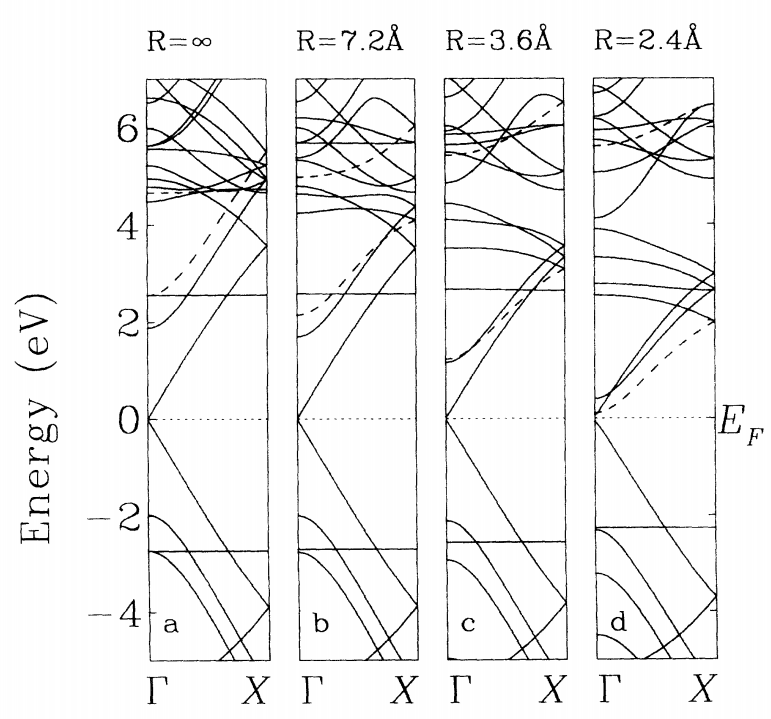
\includegraphics[scale=0.3]{images/chapter_optical_props/curvature_cnt_blase}
	\caption{Tight-binding band structure of a (6,0) nanotube as a function of nanotube diameter $R$. The Fermi level remains at 0 eV. Moreover, the presence of $\sigma^*$ and $\pi^*$ hybridization, creates two new energy bands (dashed lines) that repel each other more strongly as the nanotube radius decreases. At the lowest radius, the low energy band gets very close to the valence band. However, ab-initio calculations reveal that this low energy branch actually intersects with the valence band. Reproduced from Ref.\ \cite{blase1994hybridization}.}
	\label{fig:cnt_curvature}
\end{figure}

When $\nu= \pm 1$, the band structure corresponds to that of a medium-gap semiconductor ($\sim0.5 - 1$ eV band gap energy) \cite{nanot2012optoelectronic}. This band structure excludes the presence of a Dirac cone as shown in Figure \ref{fig:ten_zero_cnt}  \cite{charlier2007electronic}.

%\begin{figure}[h]
%	\centering
%	\begin{subfigure}{0.45\textwidth}
%		\centering
%		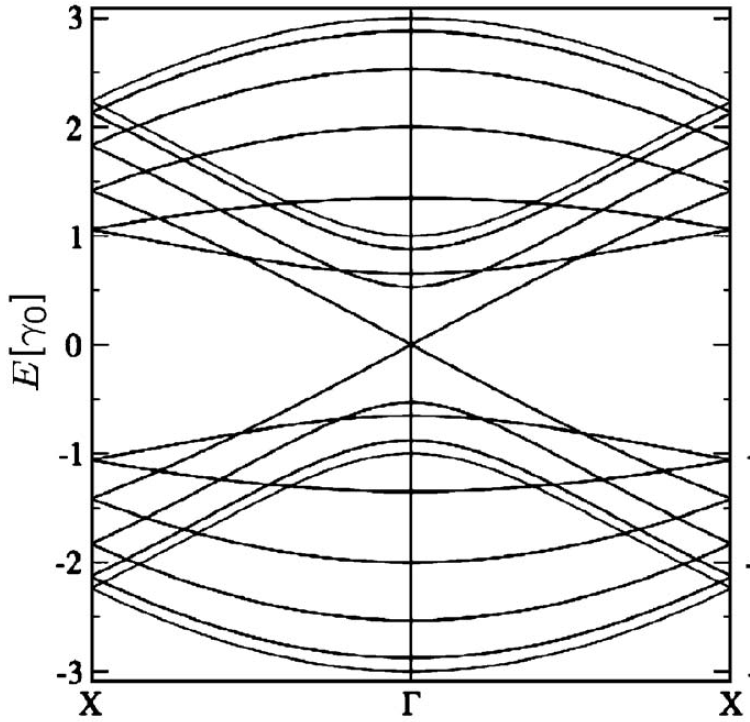
\includegraphics[scale=0.36]{images/chapter_optical_props/nine_zero_band_charlier_2}
%		\caption{Metallic}
%	\end{subfigure}
%	\qquad
%	\begin{subfigure}{0.45\textwidth}
%		\centering
%		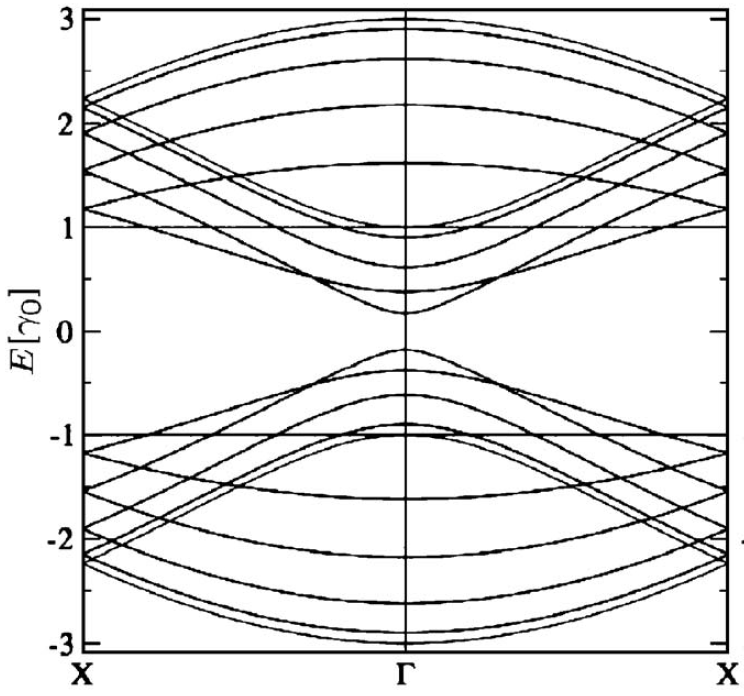
\includegraphics[scale=0.38]{images/chapter_optical_props/ten_zero_band_charlier_2}
%		\caption{Metallic}
%	\end{subfigure}
%	\caption{Reproduced and modified from Ref \cite{charlier2007electronic}.}
%\end{figure}


\begin{figure}[ht]
	\centering
	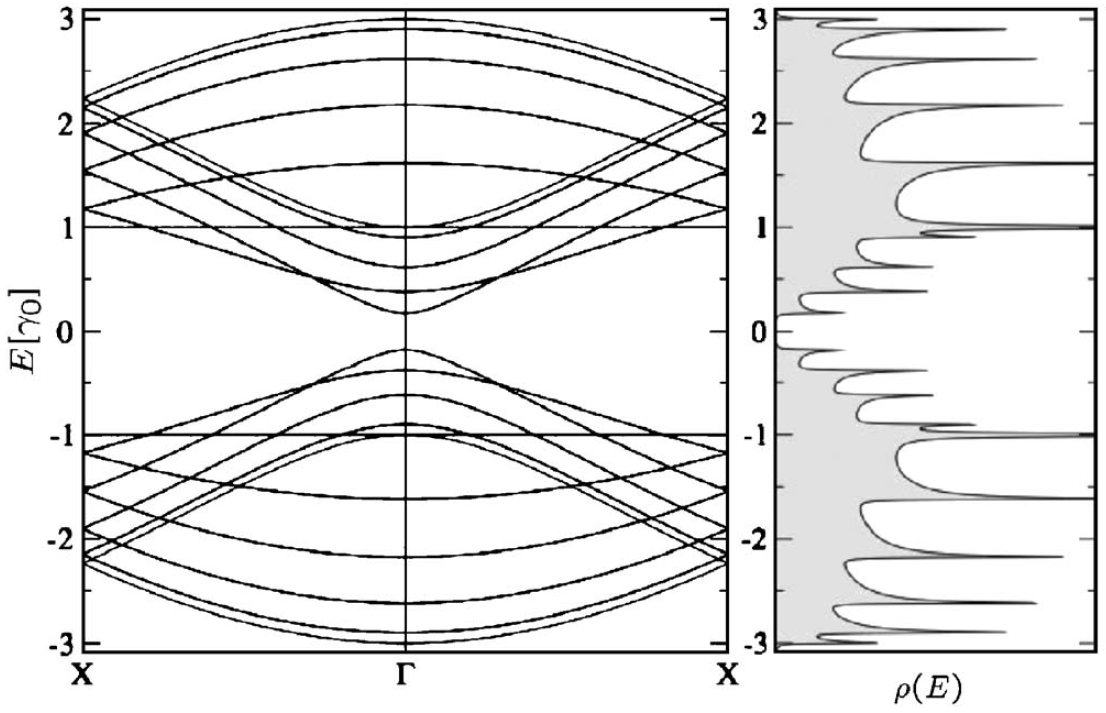
\includegraphics[scale=0.38]{images/chapter_optical_props/ten_zero_band_charlier}
	\caption{Band structure and density of states for a (10,0) carbon nanotube derived using the zone-folding scheme. These are plotted in units of $\gamma_0 \approx 2.9$ which represents the tight-binding hopping energy between first nearest-neighbors. Reproduced from \cite{charlier2007electronic}.}
	\label{fig:ten_zero_cnt}
\end{figure}


\subsection{Optical Selection Rules}
\label{section:selection_rules}
{\color{red} Explain where these come from}
Selection rules dictate the optical transitions that can occur. Such optical processes depend upon the conservation of both energy and angular momentum \cite{weismanKonoBook}.

{\color{red} UNFINISHED} Can used symmtery-based quantum numbers to get some insight regarding the selection rules. Light has zero angular momentum so $\Delta k \approx 0$ meaning that transitions occur only separated by energy in momentum-space \cite{bovzovic2000optical}
Light polarized parallel to nanotube axial direction has angular momentum $\Delta m = \pm 1$. In particular, right-handed circular polarization has $\Delta m = 1$. Whereas left-handed polarization has $\Delta m = -1$. $\sigma_\text{v}$ is symmtery group for vertical mirror reflections about xz plane. $\sigma_\text{h}$ is symmetry group for horizontal mirro reflections in xy plane. k is a quasi-momentum about z axis. m is z-component quasi-angular momentum related to the rotational symmetry.

For light polarized parallel to z-direction, parity with respect to $\sigma_\text{v}$ is preserved whereas parity with repsect to $\sigma_\text{h}$ is reversed. In other words, transitions can occur between bands that have the same parity with respect to $\sigma_\text{v}$. However, one of the bands involved in optical transition must have event parity with respect to $\sigma_\text{h}$ whilst the other band has odd parity with respect to $\sigma_\text{h}$.

In the case of light polarized perpendicular to the z-direction, parity with respect to $\sigma_\text{v}$ is reversed whereas parity with respect to $\sigma_\text{h}$ is preserved.

\begin{figure}[H]
	\centering
	\begin{subfigure}{\textwidth}
		\centering
		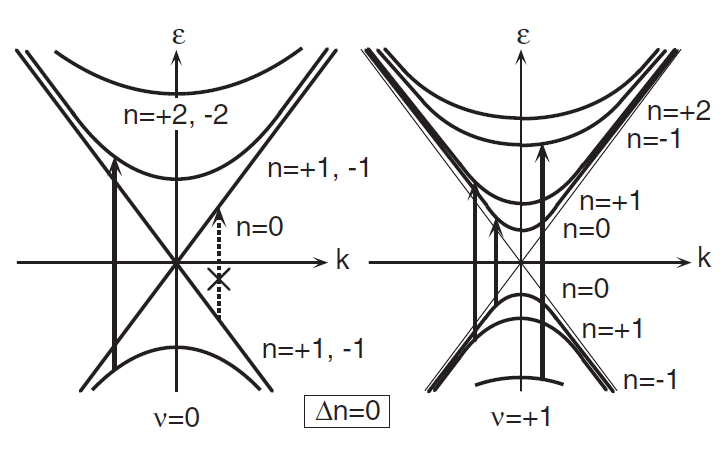
\includegraphics[scale=0.65]{images/chapter_optical_props/selection_rules_1.png}
		\caption{Selection Rules for light polarized parallel to the axial direction of carbon nanotubes. In the $\nu=0$ case, transitions within the Dirac cone are forbidden.}
	\end{subfigure}
	\begin{subfigure}{\textwidth}
		\centering
		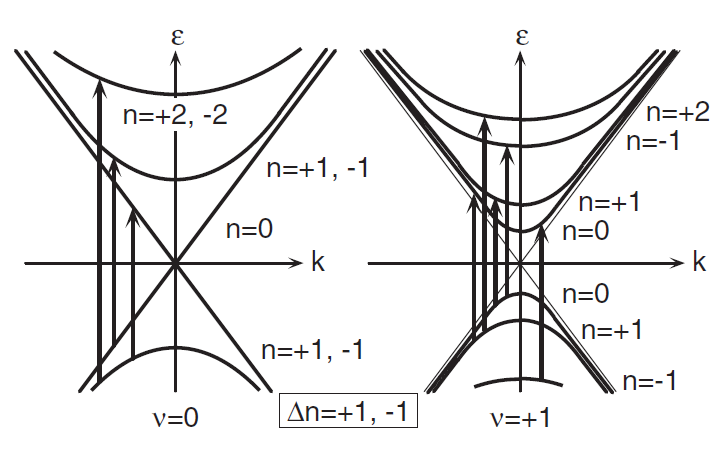
\includegraphics[scale=0.65]{images/chapter_optical_props/selection_rules_2.png}
		\caption{Selection Rules for light polarized perpendicular to the axial direction of carbon nanotubes.}
	\end{subfigure}
	\caption{Optical selection rules for metallic and narrow-gap semiconducting nanotubes ($\nu = 0 $) as well as medium-gap semiconducting nanotubes ($\nu = \pm 1$) . Reproduced from Ref.\ \cite{ando2005theory}.}
	\label{fig:selection_rules}
\end{figure}

The notation E$_{ij}$ denotes an inter-band transition between the valence sub-band $i$ and the conduction sub-band $j$ \cite{weismanKonoBook}. In addition, $\Delta n \equiv i - j$ defines the difference between the band indices $i$ and $j$.  Incident light polarized parallel to carbon nanotube axial direction excites transitions where $\Delta n = 0$ \cite{weismanKonoBook}. This includes transitions such as $E_{11}$, $E_{22}$ and $E_{33}$. Whereas, incident light polarized perpendicular to the nanotube axial direction can only excite optical transitions where $\Delta n = \pm 1$ such as $E_{12}$ \cite{weismanKonoBook}.



\section{Excitons in SWCNTs}

\subsection{Supression of Optical Transitions Involving the Free-Electron Continuum}
The simple tight-binding picture presented earlier ignores the effects of electron-electron interactions and thereby does not fully account for the effects of quantum confinement \cite{weismanKonoBook}. Indeed, the inclusion of electron-electron interactions into this picture yields a new electronic structure in which free electrons play a minimal role.

Strong electron-electron interactions influence the binding energies of quasi-particles known as excitons that form after the creation of an electron-hole pair \cite{koch2006semiconductor}. Excitons represent hydrogen-like quasi-particles composed of a negatively-charged electron bound to a positively-charged hole \cite{koch2006semiconductor}. In an ideal 1-D material, theory predicts that excitons will have an infinite binding energy \cite{ando2005theory}. This alone foreshadows the dominance of excitons in the optical properties of carbon nanotubes \cite{ando2005theory}.



The strong quantum confinement of nanotubes effectively suppresses the density of states of any free electron continuum whilst enhancing that of excitonic states. Moreover, the effective strength of Coulomb interactions $S_\text{e-e}$ can be expressed as
\begin{equation}
	S_\text{e-e} \equiv \dfrac{e^2 \kappa / L}{2 \pi \gamma / L},
\end{equation}

where $e^2 /\kappa L$ and $2 \pi \gamma / L$ account for the characteristic energy scales associated with Coulomb interactions and the kinetic energy of electrons respectively \cite{ando2005theory}. Here, $e$ defines the charge of an electron, $\gamma$ represents a band parameter, $L$ indicates the nanotube circumference $|\vec{C}_\text{h}|$, and $\kappa$ denotes the static dielectric constant used to account for screening effects.

\begin{figure}[ht]
	\centering
	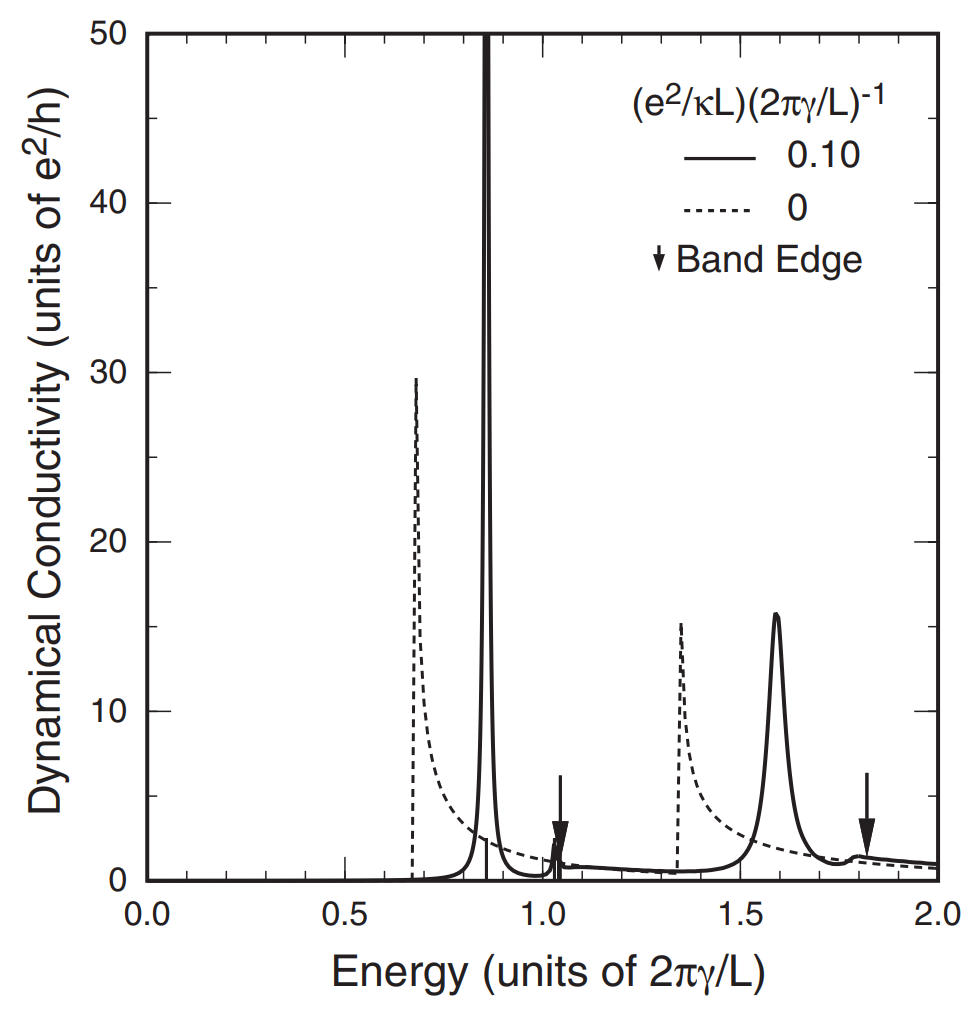
\includegraphics[scale=0.35]{images/chapter_optical_props/ando_suppression}
	\caption{Optical absorption spectrum of a semiconducting nanotube with (solid line) and without (dashed line) the effect of Coulomb interactions. Arrows mark the band edge positions of free electron continua. Reproduced and modified from Ref.\ \cite{ando2005theory}.}
	\label{fig:ando_suppression}
\end{figure}

Figure \ref{fig:ando_suppression} shows the calculated optical absorption spectrum of a semiconducting nanotube with and without the presence of Coulomb interactions. The plot shows the presence of van Hove singularities when ignoring the effect of Coulomb interactions. After accounting for these interactions, the oscillator strength of the low energy bound states of excitons becomes enhanced and absorption in the free-electron continuum drastically diminishes. The band edge of the free-electron continuum also shifts as a result of Coulomb interactions \cite{ando1997excitons}. Furthermore, this shift of the band edge increases as $S_{e-e}$ increases \cite{ando2005theory}.

\begin{figure}[ht]
	\centering
	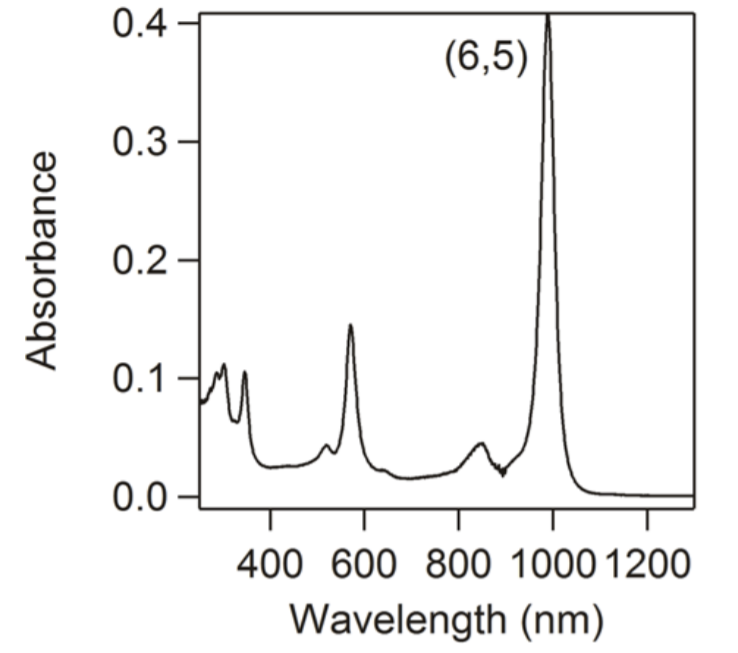
\includegraphics[scale=0.62]{images/chapter_optical_props/cnt_absorbance_yota}
	\caption{Absorbance spectrum of a (6,5) carbon nanotube sample at room temperature. The peaks at 983 and 570 nm correspond to the $E_{11}$ and $E_{22}$ of (6,5) carbon nanotubes. The $E_{12}$ transition of (6,5) nanotubes can also be observed at 650 nm. Reproduced from Ref.\ \cite{ichinose2017extraction}. }
	\label{fig:cnt_abs_yota}
\end{figure}

\subsection{Exciton Binding Energies}

In essence, the exciton binding energy characterizes the strength of the Coulomb interaction between an electron as well as its corresponding hole \cite{valkunas2006exciton}. On one hand, if the exciton binding energy is smaller than the thermal energy $k_b T$, then this Coulomb interaction becomes negligible \cite{valkunas2006exciton}. This causes electrons and holes to behave independently of each other. On the other hand, if the binding energy is much higher than the thermal energy, then electrons and holes tend to form stable, charge-neutral excitons \cite{valkunas2006exciton}.

The binding energies of excitons in CNTs tend to be on the order of hundreds of meV \cite{wang2005optical}. For instance, the excitons of (6,5) nanotubes have a binding energy of roughly 400 meV \cite{wang2005optical}. At room temperature $k_b T \approx$ 26 meV, meaning that the energy scale associated with thermal fluctuations falls short of the exciton binding energies in CNTs. Thus, excitons of CNTs are quite stable at room temperature. Figure \ref{fig:cnt_abs_yota} illustrates this effect as the room-temperature absorbance spectrum of a (6,5) sample exhibits well-defined, excitonic resonances.

Two-photon absorption measurements convincingly demonstrated that the optical transitions found in carbon nanotubes directly create excitons \cite{wang2005optical, maultzsch2005exciton}. Excitons possess a set of Rydberg states, analogous to the hydrogen atom, that can include even parity states such as 1s, 2s, and 3s as well as odd parity states such as 2p, 3p, and so on \cite{wang2005optical}. Here, the optical selection rules depend on the parity of the states involved.

For light polarized parallel to the nanotube axial direction, one-photon absorption processes require parities of the initial and final state to be opposite of each other. In contrast, two-photon absorption processes require both the initial and final state to have the same parity. The consequence of these selection rules is that one-photon excitations access excitons whose wavefunctions have even parity ($s$-symmtery) \cite{wang2005optical}. Two-photon excitation creates excitons whose wavefunctions exhibit odd parity ($p$-symmetry) \cite{wang2005optical}.

In practice, this means that one-photon absorption can access the 1$s$ exciton resonance and that two-photon absorption can access excited states above the 1$s$ exciton state as shown in Figure \ref{fig:cnt_two_photon}. Although other excited states can be accessed, these tend to have almost negligible oscillator strengths \cite{wang2005optical}. Hence, two-photon excitation can create $2p$ excitons or even free-electrons which then relax to the $1s$ exciton state before optical recombination occurs at the $1s$ exciton energy.

\begin{figure}[H]
	\centering
	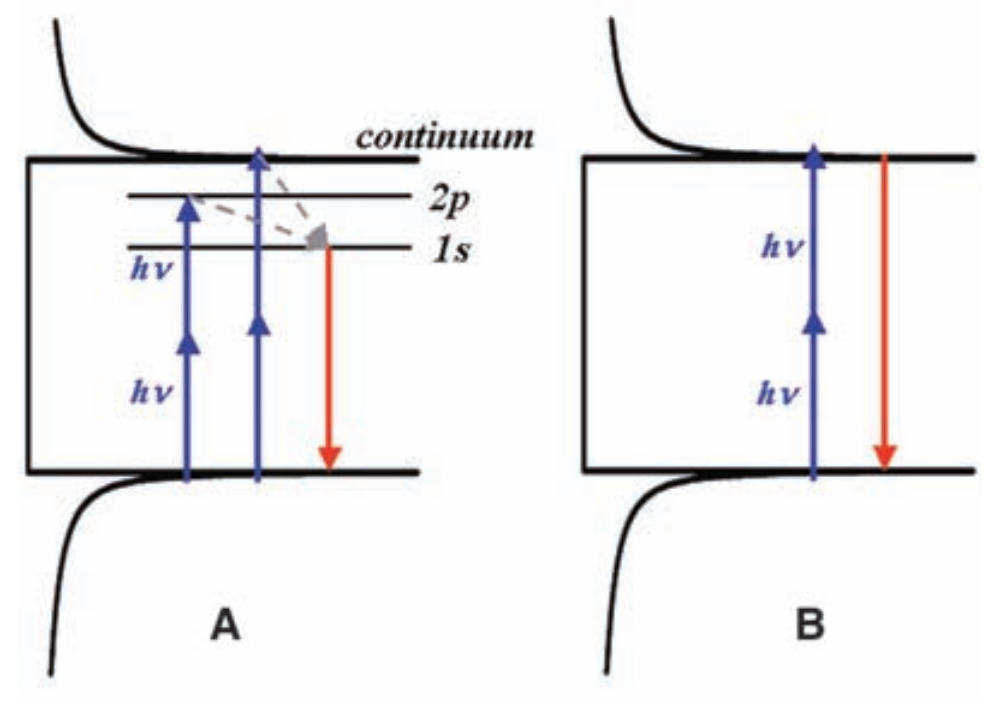
\includegraphics[scale=0.3]{images/chapter_optical_props/cnt_two_photon}
	\caption{ Two-photon absorption in the presence of electron continuum states (A) with and (B) without low lying exciton states within the band gap. When excitonic states are present, two-photon absorption can excite free electron-hole pairs or 2$p$ excitons which then decay to $1s$ excitons before optical recombination occurs. Without exciton states, photoluminescence occurs at the band gap energy from optical recombination of free electrons. Reproduced from Ref.\ \cite{wang2005optical}. }
	\label{fig:cnt_two_photon}
\end{figure}

If the tight-binding picture were correct, the optical emission would be most efficient if the two-photon excitation energy (2$\hbar \omega$) were exactly equal to the band gap energy due to the density of states associated with the van Hove singularity. The photon energy of the emission would also be equal to 2$\hbar \omega$. Figure \ref{fig:cnt_two_photon_emission} shows that optical emission instead occurs when the two-photon excitation energy is higher than photon energy of emission which supports the exciton picture in which Coulomb interactions produce strongly-correlated electron states.



\begin{figure}[H]
	\centering
	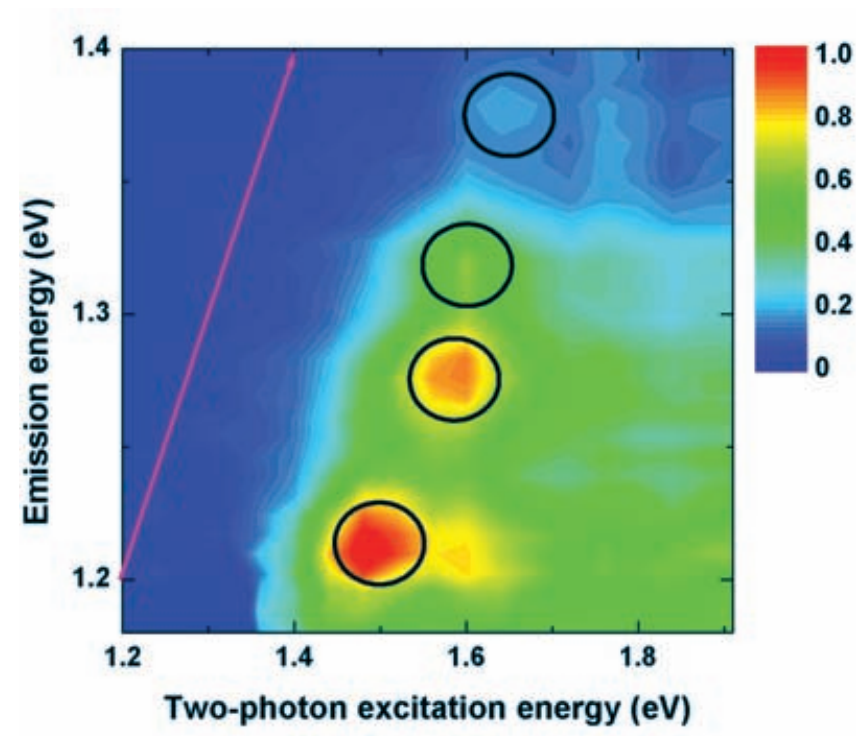
\includegraphics[scale=0.3]{images/chapter_optical_props/two_photon_wang}
	\caption{Contour plot showing emission of various SWCNTs after two-photon excitation. With increasing emission photon energy, fluorescence peaks associated with (7,5), (6,5), (8,3), and (9,1) respectively (black circles). Light emission only occurs when the two-photon exciation energy exceeds that of the emission energy. The solid line on the left-hand side shows the position where emission would occur if the tight-binding were correct. Here, the emission energy would be equal to that of the two-photon excitation energy. Reproduced from Ref.\ \cite{wang2005optical}.}
	\label{fig:cnt_two_photon_emission}
\end{figure}

Unlike carbon nanotubes, conventional semiconductors such as GaAs only exhibit excitons with binding energies typically less than 20 meV \cite{liang1970excitons}.  As a result, these materials have to be cooled down to low temperatures in order to easily observe exciton resonances as shown in Figure \ref{fig:gaas_vs_cnt_absorbance}.

\begin{figure}[h]
	\centering
	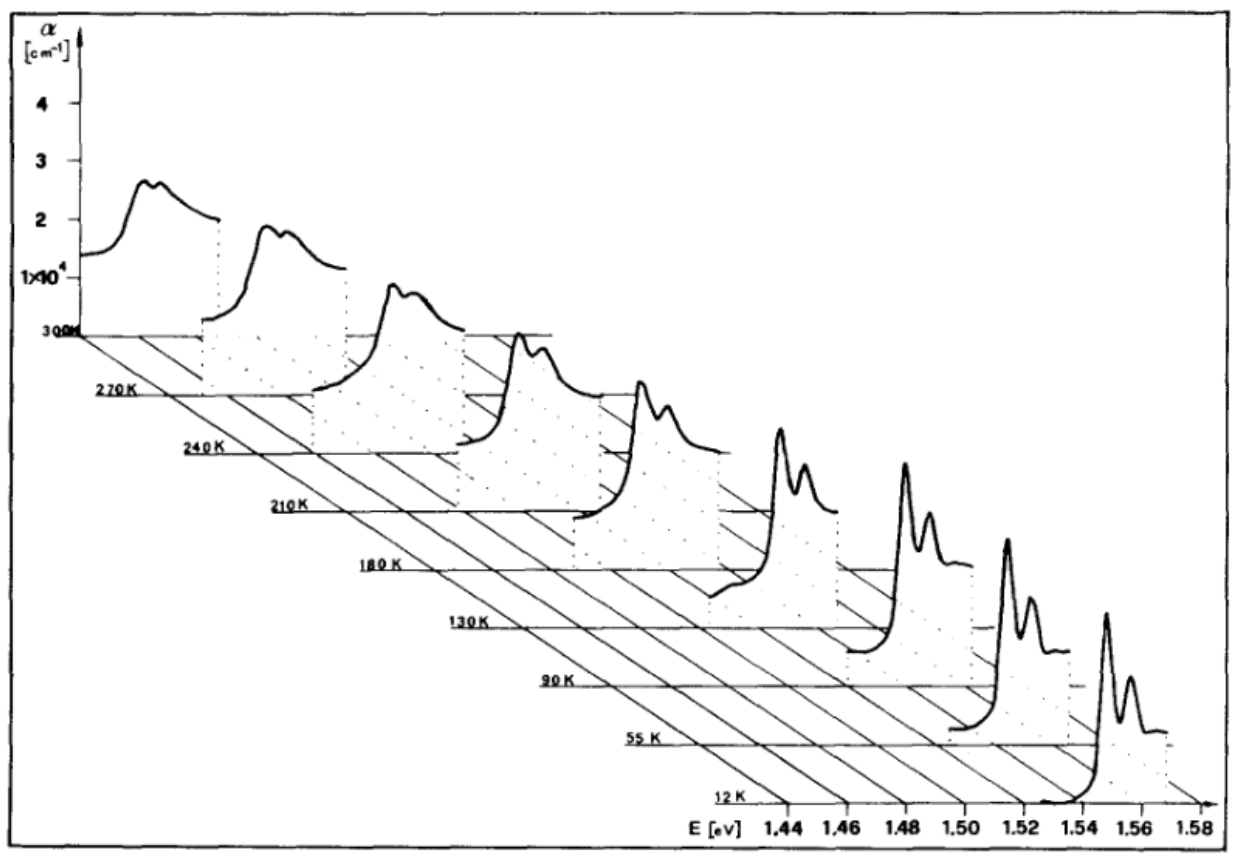
\includegraphics[scale=0.55]{images/chapter_optical_props/gaas_absorbance_filipowicz}
	\caption{GaAs/AlGaAs quantum well absorbance spectra at different temperatures. At higher temperatures, the presence of excitonic resonances is diminished. As the temperature decreases, two exciton peaks associated with light-hole and heavy-hole bands become more prominent. Reproduced from Ref.\ \cite{filipowicz1990temperature}.}
	\label{fig:gaas_vs_cnt_absorbance}
\end{figure}

\subsection{Dark and Bright Excitons}

Theory suggests that each sub-band in the band structure of carbon nanotubes possesses up to 16 excitonic states \cite{amori2018excitons}. This determination takes into account the degeneracy of the $K$ and $K'$ points in the first Brillouin zone in graphene as well as the spins of charge carriers. In addition, short-range Coulomb interactions split these 16 possible excitonic states to give rise a fine structure composed of 4 spin-singlet states and 12 spin-triplet states as shown in Figure \ref{fig:dark_bright_excitons_dispersion} \cite{srivastava2008direct}. Due to weak spin-orbit coupling, it's generally rare to convert a singlet state into a triplet state via phonon scattering processes \cite{amori2018excitons}.

Of the four singlet states, only one of these can be accessed via an optical transition and is therefore associated with every possible $E_\text{ij}$ resonance. This is commonly referred to as a ``bright" exciton state. Whereas, the remaining 3 singlet states are optically inactive meaning that they do not couple directly with light and are therefore said to be  ``dark'' states.

\begin{figure}[ht]
	\centering
	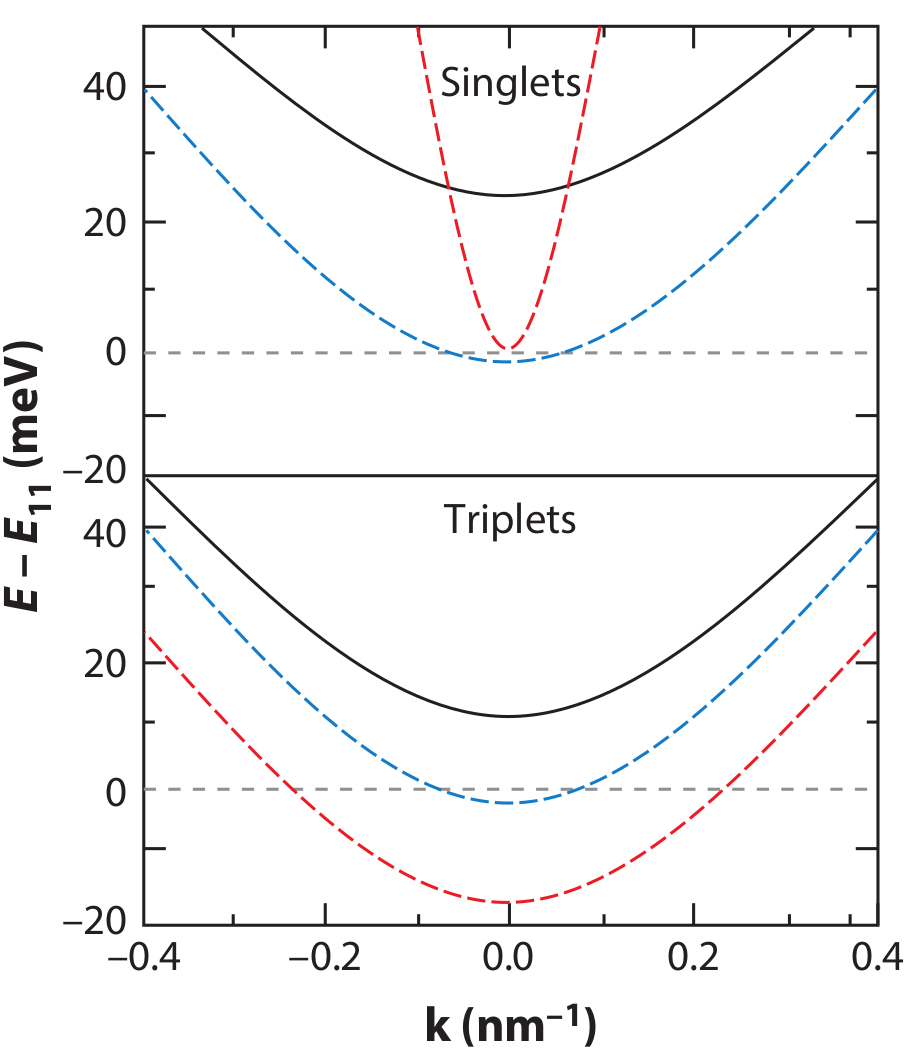
\includegraphics[scale=0.25]{images/chapter_optical_props/dark_and_bright_excitons}
	\caption{Energy dispersion of singlet and triplet states for a (19,0) nanotube. The black solid curves currespond to doubly-degenerate states with a non-zero angular moment. The red dashed curves (second highest band for singlets, and lowest band for triplets) indicate odd-parity, bright states with zero angular momentum. Finally, the blue dashed curves (lowest band for singlets and second highest band for triplets) refer to even-parity, dark states. Reproduced from Ref.\ \cite{amori2018excitons}.}
	\label{fig:dark_bright_excitons_dispersion}
\end{figure}

Additionally, Figure \ref{fig:exciton_transitions} shows a schematic diagram describing the possible electron-hole configurations for singlet states. The highest energy singlet states include charge carriers in the $K$ point bound to carriers in the $K'$ point, otherwise known as indirect excitons \cite{srivastava2008direct}. These states cannot be accessed by an optical transition as these require the change in momentum between the initial and final states to be zero.  Whereas, the lowest energy singlet states, which include a bright and a dark state, refer to electrons and holes with the same momentum that are bound together \cite{srivastava2008direct}. The lowest energy singlet state is dipole-forbidden as a result of its even-parity. Despite this, it has been observed experimentally in magneto-optical measurements.

\begin{figure}[ht]
	\centering
	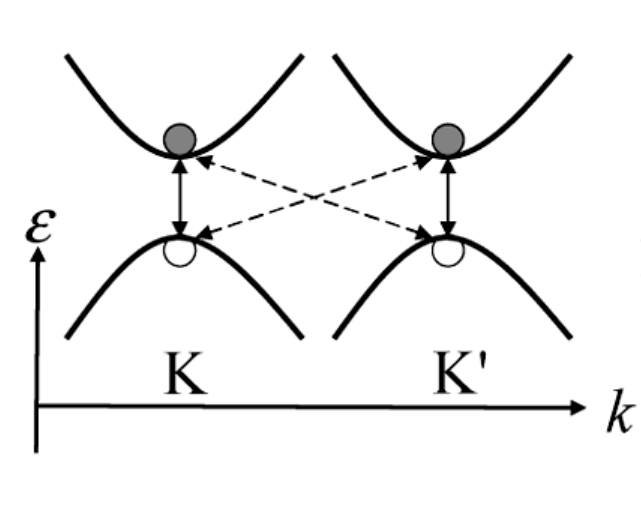
\includegraphics[scale=0.4]{images/chapter_optical_props/exciton_schematic_srivastava}
	\caption{Schematic energy dispersion for four possible spin-singlet exciton configurations. Two of these include indirect excitons appearing due to Coulomb interactions between carriers an electron (hole) in the $K$ point and a hole (electron) in the $K'$ point. The remaining two consist of excitons formed by electrons and holes with the same momentum. Reproduced from Ref.\ \cite{srivastava2008direct}.}
	\label{fig:exciton_transitions}
\end{figure}

The application of a magnetic field down the nanotube axis breaks time-reversal symmetry \cite{srivastava2008direct}. In a process known as the Aharanov-Bohm effect, the magnetic field lifts the degeneracy between $K$ and $K'$ states and brightens the dark singlet state closest in energy to the bright singlet state. Figure \ref{fig:exciton_brightening} shows illustrates the brightening of the dark exciton state in a series of magnetic field-dependent photoluminescence measurements on a single nanotube. With no magnetic field applied, the photoluminescence spectra only contains emission from the bright exciton. At higher magnetic fields, a second lower energy peak emerges due to the brightening of the dark exciton state.  

\begin{figure}[ht]
	\centering
	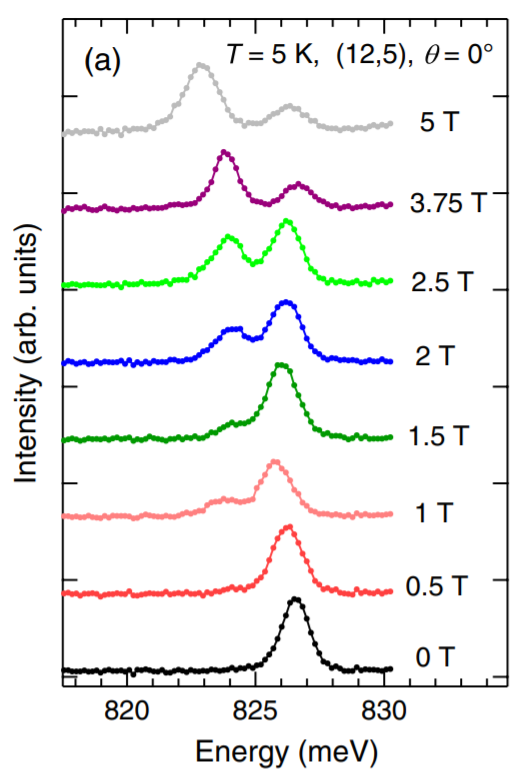
\includegraphics[scale=0.5]{images/chapter_optical_props/dark_brightening_srivastava}
	\caption{Magnetic-field dependent photoluminescence spectra obtained from a single carbon nanotube. The magnetic field is applied in a direction parallel to the nanotube axial direction. At 0 T, photoluminescnce only occurs due to the bright exciton state. At higher magnetic fields, a second emission peak appears due to the magnetic brightening of a dark exciton state as a result of the Aharonov-Bohm effect.  Reproduced from Ref.\ \cite{srivastava2008direct}.}
	\label{fig:exciton_brightening}
\end{figure}


\subsection{Phonon Side-Bands}

{\color{red} UNFINISHED} Exciton-phonon coupling \cite{perebeinos2005effect, yu2010phonon, plentz2005direct}. Absorption of light to form exciton-phonon bound state. In many nanotubes this state appears about 200 meV above the $E_{11}$ optical transition. Attributed to longitudinal optical phonon at the $K$ and $\Gamma$ points of the graphene Brillouin zone. Still conserve momentum light has negligible momentum, so we can get excitons with momentum $q$ and phonons with momentum $-q$. Suggests that exciton-phonon bound states may give indirect access to dark excitons. 

\section{Summary}

{\color{red} UNFINISHED} Carbon nanotubes exhibit unique properties. They behave as either semiconducting or metallic materials depending on their chirality $(m,n)$. Furthermore, their 1-D character establishes anisotropic optical selection rules depending on the polarization of light with respect to the carbon nanotube axial direction. Moreover, the quantum confinement imposed by their 1-D structure enhances electron-electron interactions that mitigate the oscillator strength of free-electron states in the electronic band structure. These strong Coulomb interactions promote the presence of excitons with very high binding energies that are stable even at room temperatures, unlike those of conventional semiconductors.
